\documentclass[12pt]{extarticle}
\usepackage[margin=1in]{geometry}
\usepackage{amssymb}
\usepackage{amsmath}
\usepackage{url}
\usepackage{bm}
\usepackage{color}
\usepackage{cancel}
\usepackage{verbatim}
\usepackage{fancyvrb}
\usepackage{datatool}
\usepackage{graphicx}

%My commands
\newcommand{\Oip}{\mathcal{O}^p_{i}}
\newcommand{\Oi}{\mathcal{O}_{i}}
\newcommand{\Oij}{\mathcal{O}_{ij}}
\newcommand{\Okl}{\mathcal{O}_{kl}}
\newcommand{\Oijp}{\mathcal{O}^p_{ij}}
\newcommand{\Oklp}{\mathcal{O}^p_{kl}}
\newcommand{\ket}[1]{\left| #1 \right>}
\newcommand{\bra}[1]{\left< #1 \right|}
\newcommand{\braket}[2]{\left< #1 | #2 \right>}
\newcommand{\ketbra}[2]{\left| #1 \right> \left< #2 \right|}
\newcommand{\taui}{\bm{\tau}_i}
\newcommand{\tauj}{\bm{\tau}_j}
\newcommand{\sigmai}{\bm{\sigma}_i}
\newcommand{\sigmaj}{\bm{\sigma}_j}
\newcommand{\rij}{\hat{r}_{ij}}
\newcommand{\sigmaia}{\sigma_{i\alpha}}
\newcommand{\sigmaib}{\sigma_{i\beta}}
\newcommand{\tauig}{\tau_{i\gamma}}
\newcommand{\sigmaja}{\sigma_{j\alpha}}
\newcommand{\sigmajb}{\sigma_{j\beta}}
\newcommand{\taujg}{\tau_{j\gamma}}
\newcommand{\tauij}{\taui \cdot \tauj}
\newcommand{\sigmaij}{\sigmai \cdot \sigmaj}
\newcommand{\mycolor}[1]{\textit{\textcolor{red}{#1}}}
\newcommand{\longsi}{s_1, \ldots, s_{i-1} , s, s_{i+1}, \ldots, s_A}
\newcommand{\longsij}{s_1, \ldots, s_{i-1} , s, s_{i+1}, \ldots, s_{j-1}, s', s_{j+1}, \ldots ,s_A}
\newcommand{\longsijkl}{s_1, \ldots, s_{i-1} , s'', s_{i+1}, \ldots, s_{j-1}, s''', s_{j+1}, \ldots ,s_A}
\newcommand{\Ot}{\mathcal{O}^\tau_{n\alpha}}
\newcommand{\Os}{\mathcal{O}^\sigma_{n}}
\newcommand{\Ost}{\mathcal{O}^{\sigma\tau}_{n\alpha}}
\newcommand{\detr}{\mathrm{det}}
\newcommand{\R}{\mathrm{\mathbf{R}}}
\newcommand{\subr}[1]{\color{blue}{#1}}

% sorting command
\newcommand{\sortitem}[2]{%
  \DTLnewrow{list}%
  \DTLnewdbentry{list}{label}{#1}%
  \DTLnewdbentry{list}{description}{#2}%
}

\newenvironment{sortedlist}%
{%
  \DTLifdbexists{list}{\DTLcleardb{list}}{\DTLnewdb{list}}%
}%
{%
  \DTLsort{label}{list}%
  \begin{description}%
    \DTLforeach*{list}{\theLabel=label,\theDesc=description}{%
      \item[\theLabel] \theDesc
    }%
  \end{description}% 
}

\title{Flash Cards for Quantum/Nuclear Monte Carlo}
\author{Cody L. Petrie}

\begin{document}
\maketitle

\section*{Parameters in the Code}
\begin{sortedlist}
   \sortitem{sp(s,i)}{$=\braket{s}{s_i}$}
   \sortitem{spx(s,15,i)}{$=\bra{s}\Oip\ket{s_i}$, where $p$ goes over the 15 cartesian coordinates.}
   \sortitem{d2b(s,s',ij)}{$=\frac{\braket{\Phi}{R,\longsij}}{\braket{\Phi}{RS}}$}
   \sortitem{d2bip(s,s',s'',s''',ij,kl)}{$=\frac{\braket{\Phi}{R,s_1,\ldots,s,\ldots,s',\ldots,s'',\ldots,s''',\ldots,s_A}}{\braket{\Phi}{R,S}}$ OR}
   \sortitem{f2b(s,s',ij)}{$=\sum\limits_{kop=1}^{15}f^{kop}_{ij}\bra{ss'}\mathcal{O}^{kop}_{ij}\ket{s_is_j}$}
   \sortitem{fst(3,3,ij)}{$=f$ in front of specific operator}
   \sortitem{ph(i,4,j,idet)}{$=\sum\limits_k S_{ik}\bra{k}\mathcal{O}_j\ket{s_j}$}
   \sortitem{sxz(s,i,j)}{$=\sum\limits_k S^{-1}_{jk}\braket{k}{\mathbf{r}_i,s}$}
   \sortitem{sxzi(s,i,j,iop)}{$=\sum\limits_k S'^{-1}_{jk}S'_{ki}(s)=\sum\limits_k S'^{-1}_{jk}\bra{k}\mathcal{O}^{iop}_{i}\ket{\mathbf{r}_i,s}$}
   \sortitem{sxzj(s,i,j)}{$=\sum\limits_k S''^{-1}_{jk}S''_{ki}(s)=\sum\limits_k S'^{-1}_{jk}\bra{k}\mathcal{O}^{iopjop}_{ij}\ket{\mathbf{r}_i,s}$, each $iop$ and $jop$ is looped over and added to d2b using call g2bval(d2b,sxzj,fij).}
   \sortitem{opi(s,m)}{$=\sum\limits_k S^{-1}_{mk}\bra{k}\mathcal{O}_i\ket{\mathbf{r_i},s} = \sum\limits_{s'}\mathrm{sxz(s',i,m)}\bra{s'}\mathcal{O}_i\ket{s}$}
   \sortitem{di(m)}{$=\sum\limits_k S^{-1}_{mk}\bra{k}\mathcal{O}_i\ket{\mathbf{r_i},s_i} = \sum\limits_s \mathrm{opi(s,m)}\braket{s}{s_i}$}
   \sortitem{sx15(s,15,i,j)}{$=\sum\limits_k S^{-1}_{jk}\bra{k}\sum\limits_{kop=1}^{15}\mathcal{O}_{kop}\ket{\mathbf{r},s} = \mathrm{opmult(sxz0)}$, where sx15(:,kop,:,k) = opi(s,k)}
   \sortitem{\subr{sxzupdate(sxznew(out),detrat(out),sxzold,i,opi,sp)}}{Here the outputted detrat is simply di(i).}
   \sortitem{\subr{vnpsi2(w,dopot)}}{This subroutine ...???}
   \sortitem{\subr{hspot(???)}}{???}
   \sortitem{d15(kop)}{=di(i)$=\sum\limits_k S^{-1}_{ik}\bra{k}\mathcal{O}_i\ket{\mathbf{r},s_i} = (S'/S)_{ii}$ for a specific kop (1 of 15)}
   \sortitem{\subr{opmult(sp)}}{This multiplies sp(s,i) by the 15 operators in this order 1-3 sx,sy,sz, 4-6 tx,ty,tz, 7-9 sx*(tx,ty,tz), 10-12 sy*(tx,ty,tz), 13-15 sz*(tx,ty,tz). This outputs opmult(s,kop,i)}
   \sortitem{\subr{g2bval(d2b,sxz,fij)}}{Given sxz this computes the d2b terms.}
   \sortitem{\subr{op2val(d2b,sp,spx)}}{???}
   \sortitem{tau(3,3,npair)}{I think the 3 is x,y,z.}
   \sortitem{sigma(3,3,npair)}{I think the 3 is x,y,z.}
   \sortitem{sigtau(3,3,3,3,npair)}{I think the 3 is x,y,z.}
   \sortitem{tz(s,s')}{=spx(s,$\tau_\alpha$,i)*spx(s',$\tau_\alpha$,j)$=\bra{s,s'}\tau_{\alpha i}\tau_{\alpha j}\ket{s_i s_j}$}
   \sortitem{sz(s,s')}{=spx(s,$\sigma_\alpha$,i)*spx(s',$\sigma_\beta$,j)$=\bra{s,s'}\sigma_{\alpha i}\sigma_{\beta j}\ket{s_i s_j}$}
   \sortitem{stz(s,s')}{=spx(s,$\sigma_\alpha\tau_\gamma$,i)*spx(s',$\sigma_\beta\tau_\gamma$,j)$=\bra{s,s'}\sigma_{\alpha i}\tau_{\gamma i}\sigma_{\beta j}\tau_{\gamma j}\ket{s_i s_j}$}
\end{sortedlist}

\section*{Variational Monte Carlo}
\textbf{Steps for Metropolis Algorithm:}
\begin{enumerate}
   \item{Start with some random walker configuration $\R$}
   \item{Propose a move to a new walker $\R'$ from the distribution $T(\R'\leftarrow\R)$}
   \item{The probability of accepting the move is given by \[A(\R'\leftarrow\R) = \mathrm{min}\left(1,\frac{T(\R'\leftarrow\R)P(\R')}{T(\R'\leftarrow\R)P(\R)}\right).\] The move is accepted if $U[0,1]<A(\R'\leftarrow\R)$.}
   \item{Repeat from step 2.}
\end{enumerate}
\textbf{Variational Energy (In terms of $E_L(\R)$ and $P(\R)$), x2 + $E_L$ and $P$:}
\begin{align*}
   E_V = \frac{\int\Psi^*(\R)\hat{H}\Psi(\R)d\R}{\int\Psi^*(\R)\Psi(\R)d\R} = \int P(\R)E_L(\R)d\R \\ P(\R) = |\Psi_T(\R)|^2/\int |\Psi_T(\R)|^2d\R\ \\ E_L(\R) = \Psi_T^{-1}(\R)\hat{H}\Psi_T(\R)
\end{align*}
\textbf{Sampled Variational Energy:}
\begin{equation*}
   E_V \approx \frac{1}{N}\sum\limits_{n=1}^N E_L(\R_n)
\end{equation*}
where $\R_n$ are drawn from $P(\R)$.

\section*{General Physics}
\textbf{Atomic Shell Model}
\begin{itemize}
   \item \textbf{Shells} are areas in which an electron can "orbit" a nucleus. They correspond to the principle quantum numbers (n=1,2,3,4,...) where n=1 is the closest shell.
   \item The number of allowed electrons is controlled by the spin statistics the other allowed quantum numbers being l=0,1,...,n-1 and ml=-l,...,l. The number allowed for each shell is all the possible times two since ms=-1/2,1/2.
   \item \textbf{Subshells} are given by the l quantum numbers where l=1,2,3,4 are s,p,d,f,g.
   \item List of how many each shell can hold
   \begin{figure}[h!]
      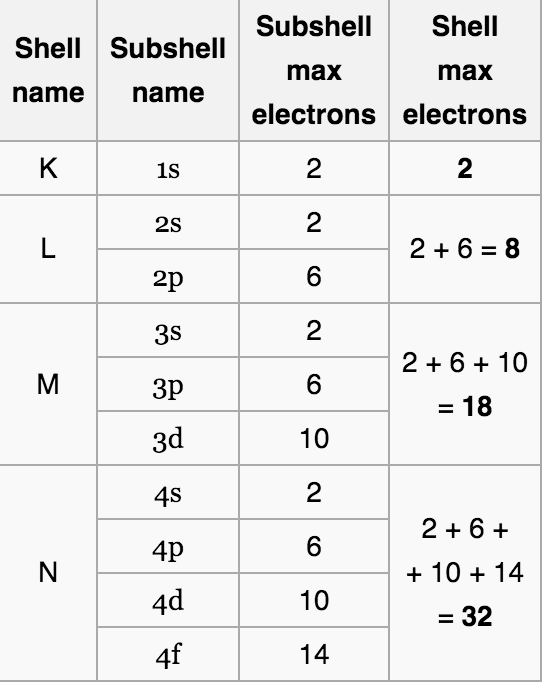
\includegraphics[width=0.25\textwidth]{shell.png}
   \end{figure}
\\
\textbf{Nuclear Shell Model} \\
The nuclear shell model is similar to the atomic shell model except that n=1,2,3,4,... and l=0,1,2,3,... independently from n. So you can have states like 1g
   
\end{itemize}

\end{document}
